\documentclass{standalone}
\usepackage{tikz}
\usetikzlibrary{patterns, angles}

\begin{document}
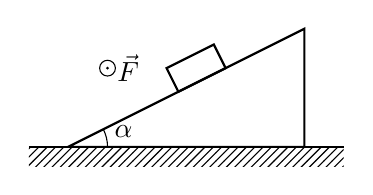
\begin{tikzpicture}
	\coordinate (A) at (0.5, 0);
    \coordinate (B) at (3.5, 0);
    \coordinate (C) at (3.5, 1.5);
       
	\draw [draw=none, pattern=north east lines] (0,-0.25) rectangle (4, 0);	
	\draw [thick] (0, 0) -- (4, 0);

	\draw [thick] (A) -- (B) -- (C) -- cycle;
	\draw [thick] (1.9,0.7) -- (2.5, 1.0) -- (2.35,1.3) -- (1.75, 1.0) --  cycle;	

	\draw [fill] (1,1) circle (0.01);
	\draw (1,1) circle (0.1) node [right] {$\vec{F}$};
	\pic [draw, -, angle eccentricity=1.5] {angle = B--A--C};
	\node [right=20pt, above] at (A) {$\alpha$};
\end{tikzpicture}
\end{document}